\documentclass[12pt,a4paper]{article}
\usepackage[T1]{fontenc} 
\usepackage[a4paper]{geometry}
\usepackage[brazil]{babel}
\usepackage[utf8]{inputenc}
\usepackage{setspace}
\usepackage{libertine}
 
\usepackage{url}

\usepackage{hyperref}

\usepackage{cite}  % Needed to use citations.

\usepackage{color,graphicx}
\usepackage{xcolor} 
 
\title{Os meios de comunicação como extensões do homem}
%\author{Humberto Lino Dias \\  \href{mailto:hldtux@gmail.com}{hldtux@gmail.com} }
%\author{Humberto Lino Dias \\ hldtux@gmail.com}
\author{Humberto Lino Dias}
 
\begin{document}
\maketitle
\abstract{In this article we review some chapters of the book \emph{Understanding Media: The Extensions of Man}, giving you a short and direct assessment of its contents.}
\pagenumbering{gobble}
\singlespacing
 
 
\section{Resenha do Livro}

\begin{center}

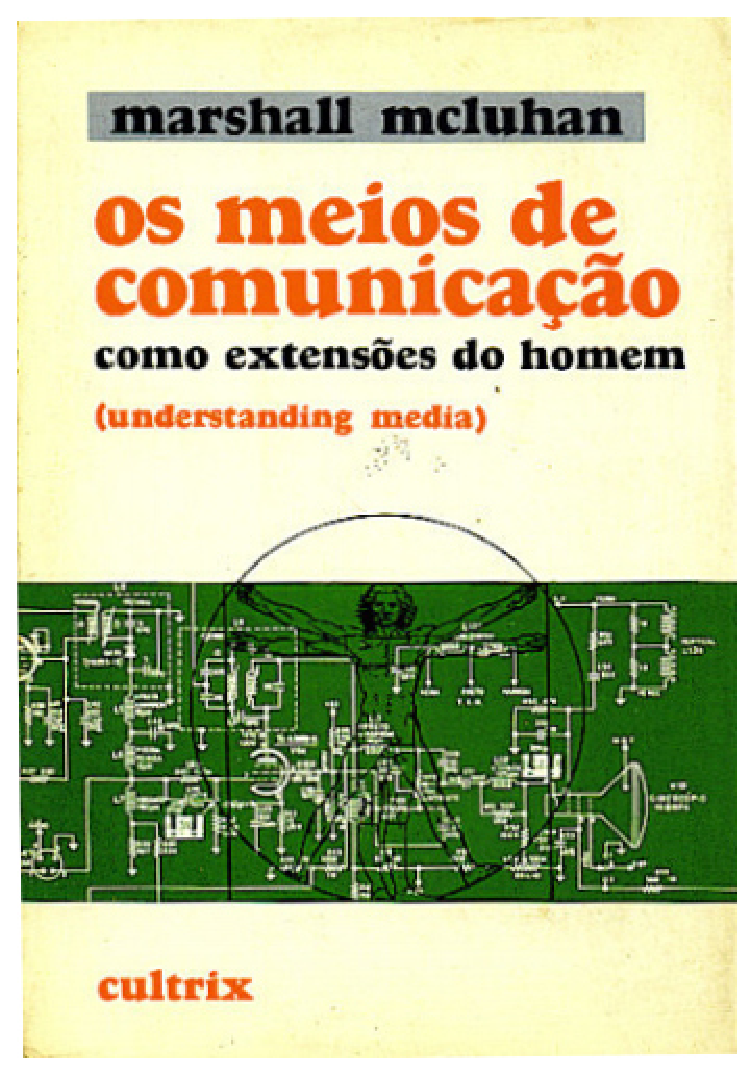
\includegraphics[height=3.1in]{book_cover.eps} \\ [1em]
\textbf{Obra}: McLuhan, Marshall - Os meios de Comunicação como Extensões do Homem, 5 ed. Editora Cultrix São Paulo, 1979. \cite{understanding_media}

\end{center}

 
\subsection{Sobre a obra}
 
\paragraph{}
O Livro ``Os meios de comunicação como extensões do homem''\cite{understanding_media} que tive acesso é dividido em duas partes. A primeira com sete capítulos e a segunda com 26 capítulos. Foi lançado em 1964 e contém uma teoria interessante e inovadora para sua época. No primeiro capítulo o teórico da comunicação e autor do mesmo \textbf{Marshall McLuhan}\cite{wiki:marshall_mcluhan}, defende sua teoria de que os meios de comunicação são, como qualquer outra tecnologia, extensões do corpo humano.
Inclusive citando exemplos como óculos que são extensões dos olhos humanos. Assim como os carros são dos pés e pernas, as roupas da pele, os livros da memória, os veículos de comunicação também aceleram e ampliam nossa comunicação verbal e visual. Tanto que essa metáfora dá nome ao seu livro.
\paragraph{}
Nos capítulos seguintes ele divide a evolução dos meios de comunição \cite{youtube:abc_monday_conference} em três grandes fases, inclusive para representar a grande distância entre elas, as nomeou de galaxias, são elas:

\subsection{Oral}
\paragraph{}
Nesta fase, toda a comunicação era feita apenas pela fala, o que tornava o \hyphenation{co-nhe-ci-men-to} restrito aos grupos que se comunicavam com a mesmo dialeto. Além de ser uma comunicação de meio ruidoso. Ou seja, quanto mais a mensagem trafega, mais ela se distancia da versão original. Característica que não ocorre na galáxia seguinte.

\subsection{Tipográfica}

\paragraph{}
É marcada pelo início da prensa de \textbf{Gutenberg}.
Com ela a cultura e o conhecimento puderam então, serem passadas adiante de forma direta.
Para Mcluhan, a imprensa é o livro diário das pessoas e ele atribui à ela o crescimento do nacionalismo. 
Mesmo não sendo ruidosa, ainda existiam barreiras linguísticas, que foram sobrepostas pela linguagens regionais da imprensa.

\subsection{Eletrônica}
\paragraph{}
O avanço significativo da tecnologia permitiu que todo o conhecimento ficasse disponível e com fácil acesso.
Sendo a comunicação instantânea e a velocidade com que as informações são passadas é incrivelmente alta.
Uma crítica que Mcluhan\cite{wiki:marshall_mcluhan} faz, é que com o acesso rápido e fácil ao conhecimento, as pessoas não se esforçam tanto para memorizar como antes. \cite{ted:ted_talk_feats_of_memory_anyone_can_do}
Mcluhan também fala sobre os novos meios de comunicação.
Segundo ele, as novas mídias situam certas personalidade em um novo plano de existência.
O que cada uma dessas personalidade faz, se torna ponto de consciência coletiva para uma sociedade inteira.

\paragraph{}
Por fim, o autor nos capítulos seguintes,  reforça ainda mais sua teste. A expandindo no contexto global, com a referência a globalização da Aldeia Global.
Mcluhan comenta o surgimento do cinema, do rádio e da televisão trouxeram de volta os meios quentes para protagonizar outra revolução. Nesse ponto de transição, Marshall McLuhan\cite{wiki:marshall_mcluhan} estuda os acontecimentos e faz projeções para o futuro. 
Ele percebe que o modelo educacional seria ultrapassado e que os limites de espaços-temporais seriam ainda mais dilatados e que passaríamos a ter grande parte das experiências sensoriais atraves
de meios, vivendo assim em um mundo virtual. Outro aspecto foi inspirado nas comunidades tribais, em que o conhecimento era passado oralmente, sem a pressuposição inerente da escrita de racionalizações e linearidades. Com esse entendimento de que a sociedade ocidental voltaria a ter aspectos de uma aldeia, mas escala mundial, surge o conceito da Aldeia global.
Aproveitando a menção ao termo global, podemos associar segundo o novo conceito de meio que abordamos acima, no cenário nacional do país. A rede globo é o meio/veículo que transmite mensagens e mensagens para o grande público os \textbf{receptores}.
 
\bibliography{refs}
\bibliographystyle{plain}
 
\end{document}